\subsection{Exercises}

%%%%%%%%%%%%%%%%%%%%%%%%%%%%%%%
\Large{Problem 2.1}
\label{ex:ex21}

\begin{figure}[H]
        \centering
        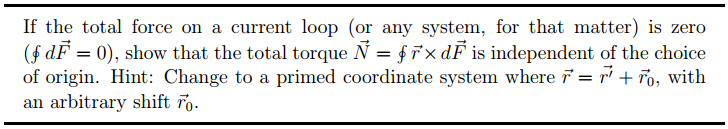
\includegraphics[width=0.8\textwidth,keepaspectratio]{prbl21}
        \label{fig:prbl21}
\end{figure}

\textit{Remember:}
\begin{itemize}
	\item Zero total force means zero change in the total momentum (conservation 
of momentum).
	\item Rotations can arise (about the centre of mass) from forces applied off centre, even 
	when the vector sum of all forces cancels out.
	\item The total torque is independent of the choice of origin.
\end{itemize}

\begin{align*}
\oint d\vec{F}  = 0 \\
\vec{N}  = \oint \vec{r} \times d\vec{F} \\
\vec{r}  = \vec{r'} + \vec{r_{0}}
\end{align*}

%\begin{proof}
\textit{Proof.}
\begin{align*}
\vec{N'} & = \oint (\vec{r} - \vec{r_{0}}) \times d \vec{F} \\ 
\vec{N'} & = \oint \vec{r} \times d\vec{F} - \oint \vec{r_0} \times d\vec{F} \\
\end{align*}
\[
\begin{rcases*}
\vec{N'} = \oint \vec{r} \times d\vec{F} - \vec{r_0} \times \oint d\vec{F} \\
\text{We know that: } \oint d\vec{F} = 0 \\
\end{rcases*} \vec{N'} = \oint \vec{r} \times d\vec{F} = \vec{N}
\]
%\end{proof}

\clearpage

%%%%%%%%%%%%%%%%%%%%%%%%%%%%%%%
\Large{Problem 2.2}
\label{ex:ex22}

\begin{figure}[H]
        \centering
        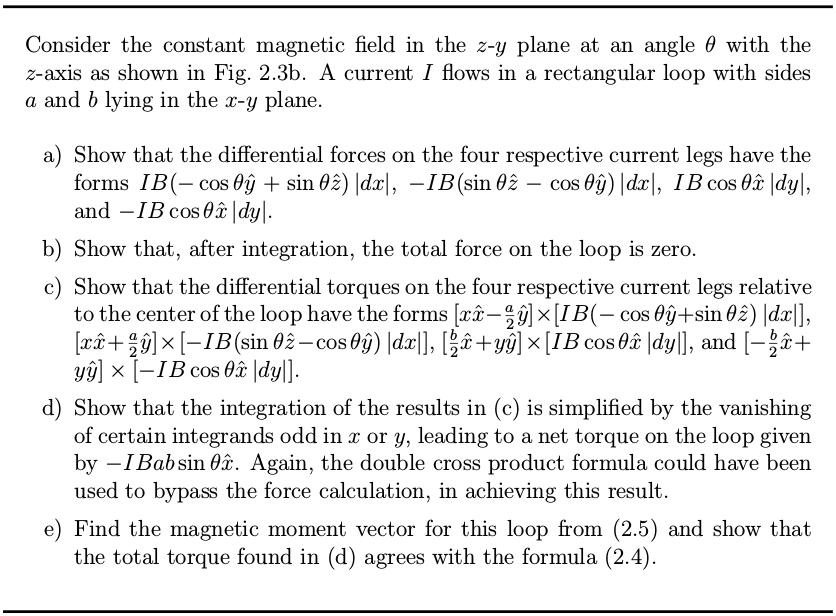
\includegraphics[width=0.8\textwidth,keepaspectratio]{prbl22}
        \label{fig:prbl22}
\end{figure}

\begin{figure}[H]
        \centering
        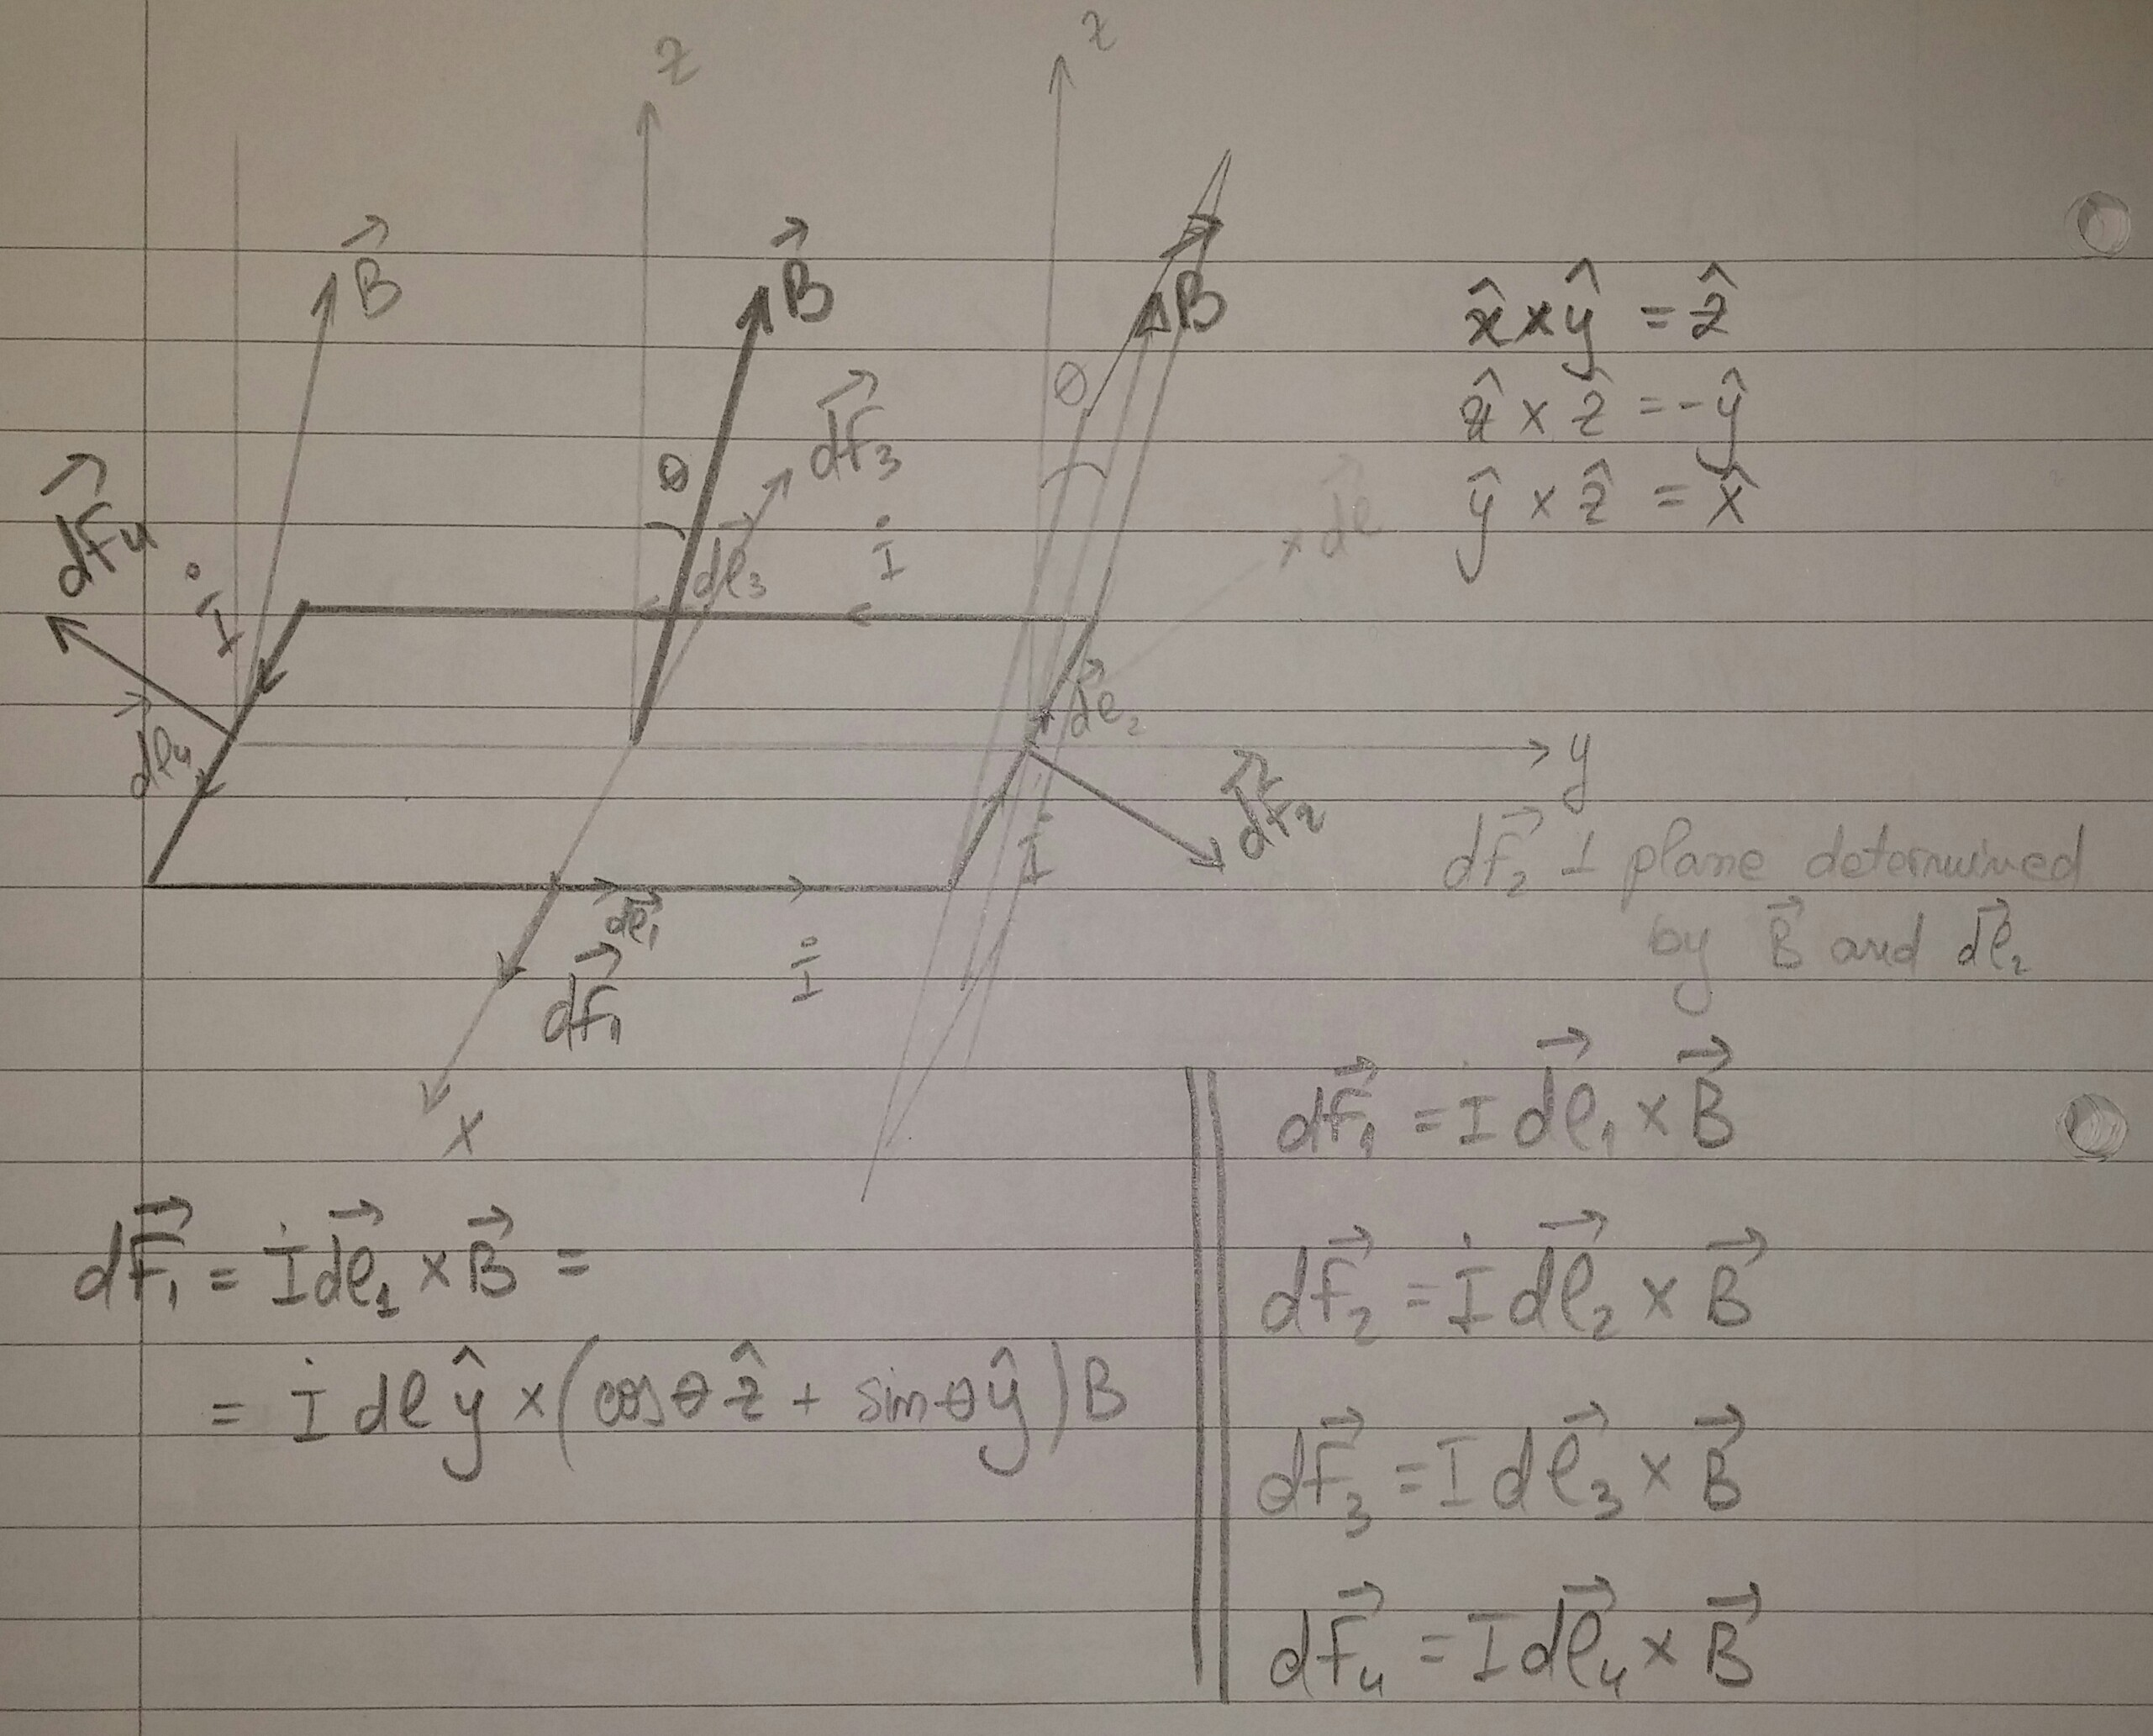
\includegraphics[width=.9\textwidth,keepaspectratio]{problem22}
        \label{fig:problem22}
\end{figure}

\textit{Remember:}
\begin{itemize}
	\item A rectangular loop behaves in a similar fashion as a 
	circular one.
	\item The total force on the loop is zero.
	\item The total torque depends on the dimensions of the loop.
\end{itemize}

\begin{wrapfigure}{r}{0.4\textwidth}
  \begin{center}
    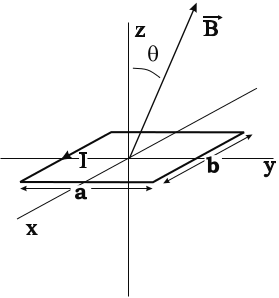
\includegraphics[width=0.38\textwidth]{fig23b}
  \end{center}
  \caption{current loops lying in the x-y plane and a magnetic charge pair along the z-axis}
\end{wrapfigure}

\textit{We know:}\\
\begin{flalign*}
    \hat{x} \times \hat{y} &= \hat{z} \\
    \hat{x} \times \hat{z} &= - \hat{y} \\
    \hat{y} \times \hat{z} &= - \hat{x} \\ \\
    \vec{B} &= \vec{B_y} + \vec{B_z} \\
    \vec{B} &= (cos \theta \hat{z} + sin \theta \hat{y})B
\end{flalign*}

\textit{a) Proof.}\\ \\
A current I flowing through a loop placed in an external magnetic field B will experience a differential force on the loop determined by:
\begin{equation} 
    d\vec{F} = I d\vec{l} \times \vec{B} \\ \\ %\Longrightarrow \\ \\
\end{equation}

As this loop has a rectangular shape, each side of the loop will experience a differential force determined by its respective differential segments. These differential segments $d\vec{l}$ will 

We get:
\begin{flalign*}
d\vec{F_{1}} &= I \vec{dl_1} \times \vec{B} \\
             &= I \abs{dl} \hat{y} \times (cos \theta \hat{z} + sin \theta \hat{y}) B \\
             &= I B cos\theta \hat{x} \abs{dl} \\
d\vec{F_{2}} &= I \vec{dl_2} \times \vec{B} \\
             &= - I \abs{dl} \hat{x} \times (cos \theta \hat{z} + sin \theta \hat{y}) B \\
             &= I B cos\theta \hat{y} \abs{dl} - I B sin\theta \hat{z} \abs{dl} \\
d\vec{F_{3}} &= I \vec{dl_3} \times \vec{B} \\
             &= - I \abs{dl} \hat{y} \times (cos \theta \hat{z} + sin \theta \hat{y}) B \\
             &= - I B cos\theta \hat{x} \abs{dl} \\
d\vec{F_{4}} &= I \vec{dl_4} \times \vec{B} \\
             &= I \abs{dl} \hat{x} \times (cos \theta \hat{z} + sin \theta \hat{y}) B \\
             &= - I B cos\theta \hat{y} \abs{dl} + I B sin\theta \hat{z} \abs{dl}
\end{flalign*}


\textit{b) Proof.}
\begin{align*}
\vec{F} &= d\vec{F_1} + d\vec{F_2} + d\vec{F_3} + d\vec{F_4} \\
\vec{F} &= I B cos\theta \hat{x} \abs{dl} 
         + I B cos\theta \hat{y} \abs{dl} 
         - I B sin\theta \hat{z} \abs{dl} \\
        &- I B cos\theta \hat{x} \abs{dl}
         - I B cos\theta \hat{y} \abs{dl} 
         + I B sin\theta \hat{z} \abs{dl}\\
& = 0
\end{align*}

\textit{c) Proof.}
\begin{align*}
    d\vec{N_i} &= \vec{r_i} \times d\vec{F_i} \\ \\
    \vec{r_1} &= \frac{b}{2} \hat{x} + y \hat{y} \\
    \vec{r_2} &= x \hat{x} + \frac{a}{2} \hat{y} \\
    \vec{r_3} &= - \frac{b}{2} \hat{x} + y \hat{y} \\
    \vec{r_2} &= x \hat{x} - \frac{a}{2} \hat{y} \\ \\
    d\vec{N_1} &= (\frac{b}{2} \hat{x} + y \hat{y}) \times (I B cos\theta \hat{x} \abs{dl}) \\ 
               &= -IBcos\theta y \abs{dl} \hat{z} \\
    d\vec{N_2} &= (x \hat{x} + \frac{a}{2} \hat{y}) \times (I B cos\theta \hat{y} \abs{dl} - I B sin\theta \hat{z} \abs{dl}) \\ 
               &= IBcos\theta x \abs{dl} \hat{z}  - IBsin\theta\abs{dl} (-x\hat{y} + \frac{a}{2}\hat{x}) \\
    d\vec{N_3} &= (- \frac{b}{2} \hat{x} + y \hat{y}) \times (- I B cos\theta \hat{x} \abs{dl}) \\ 
			   &= IBcos\theta y \abs{dl} \hat{z} \\
    d\vec{N_4} &= (x \hat{x} - \frac{a}{2} \hat{y}) \times (- I B cos\theta \hat{y} \abs{dl} + I B sin\theta \hat{z} \abs{dl}) \\ 
			   &= -IBcos\theta x \abs{dl} \hat{z}  + IBsin\theta\abs{dl} (-x\hat{y} - \frac{a}{2}\hat{x}) \\
\end{align*}

\textit{d) Proof.}
\begin{align*}
\vec{N} &= \int_{-a/2}^{a/2} d\vec{N_1} + \int_{-b/2}^{b/2} d\vec{N_2} 
         + \int_{-a/2}^{a/2}d\vec{N_3} + \int_{-b/2}^{b/2}d\vec{N_4} \\
        &= \int_{-a/2}^{a/2} d\vec{N_1} + d\vec{N_3} + \int_{-b/2}^{b/2} d\vec{N_2} + d\vec{N_4} \\
        &= 0 + \int_{-b/2}^{b/2} IBsin\theta\abs{dl} (\cancel{-x\hat{y}} - \frac{a}{2}\hat{x} \cancel{+ x\hat{y}} - \frac{a}{2}\hat{x}) dx \\
        &= -IB ab \ sin\theta \hat{x}
\end{align*}

\textit{e) Proof.}
\begin{align*}
\vec{N} &= \vec{\mu} \times \vec{B} \\
        &= I A \ \hat{n} \times \vec{B} \\
        &= I ab \ \hat{n} \times \vec{B} \\
        &= - I B ab \ sin\theta \hat{x}\\
\end{align*}


\clearpage
%%%%%%%%%%%%%%%%%%%%%%%%%%%%%%%
\Large{Problem 2.3}

\begin{figure}[H]
        \centering
        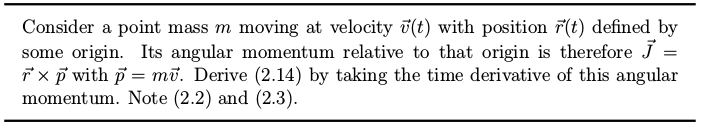
\includegraphics[width=0.8\textwidth,keepaspectratio]{prbl23}
        \label{fig:prbl23}
\end{figure}

\textit{Remember:}
\begin{itemize}
	\item A magnetic moment will try to line up along the direction of 
	an external magnetic field.
	\item If the system has nonzero total torque $\vec{N}$, then the 
	system's total angular momentum $\vec{J}$ changes according to 
	$\frac{d\vec{J}}{dt} = \vec{N}$.
\end{itemize}

(2.14) $\frac{d\vec{J}}{dt} = \vec{N}$ \\ \\
(2.2) $\vec{F} = \frac{d\vec{p}}{dt}$ \\ \\
(2.3) $d\vec{N} = \vec{r} \times d\vec{F}$.\\  \\
\textit{Proof.}
\begin{align*}
    \vec{J} & = \vec{r} \times \vec{p} \\
    \frac{d\vec{J}}{dt} & = \frac{d\vec{r}}{dt} \times \vec{p} + \vec{r} \times \frac{d\vec{p}}{dt} \\
    & = \vec{v} \times \vec{p} + \vec{r} \times \vec{F} \\
    & = \vec{v} \times (m \cdot \vec{v} ) + \vec{r} \times \vec{F} \\
    & = \mathbf{0} + \vec{N} = \vec{N}
\end{align*} 

\clearpage
%%%%%%%%%%%%%%%%%%%%%%%%%%%%%%%
\Large{Problem 2.4}

\begin{figure}[H]
        \centering
        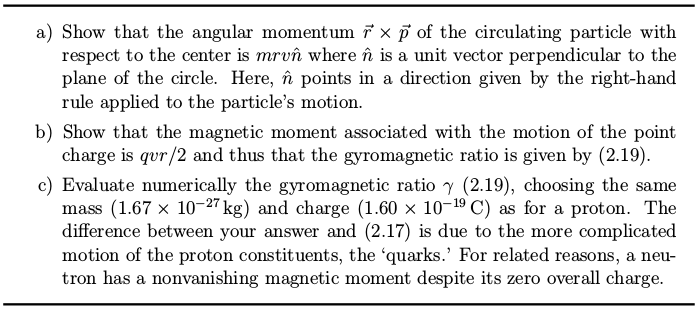
\includegraphics[width=0.8\textwidth,keepaspectratio]{prbl24}
        \label{fig:prbl24}
\end{figure}

\textit{Remember:}
\begin{itemize}
	\item The relationship between angular momentum and magnetic 
	moment is given by $\vec{\mu} = \gamma \vec{J}$
	\item In classic terms, the angular momentum depends on the mass 
	and velocity of the circulating particle.
	\item The current $I = \frac{q}{t}$ is the flux of charge in time.
	\item There are differences due to mass between different types of 
	of circulating particles.
\end{itemize}

\textit{a) Proof.}
\begin{align*}
    \vec{r} \times \vec{p} & = \vec{r} \times (m \cdot \vec{v}) \\
    & = m r v \ sin\theta \hat{n}\\
    \text{ with } \theta & = 90^0 \Rightarrow \\
    \vec{r} \times \vec{p} & = m r v \hat{n}
\end{align*}

\textit{b) Proof.}
\begin{align*}
	\vec{\mu} &= \gamma \vec{J} \\
	          &= \gamma \vec{r} \times \vec{p} \\
	          &= \gamma m r v \hat{n}\ (1) \\
	\vec{\mu} &= I A \hat{n} \\
	          &= \frac{q}{T} \ \pi r^2 \hat{n} \\
	          &= \frac{q \, v}{2 \cancel{\pi} \cancel{r}} \ \cancel{\pi} 
	          r^{\cancel{2}} \hat{n}  \\
	          &= \frac{qvr}{2} \, \hat{n} \, (2)
\end{align*}
\begin{align*}
\text{From (1) and (2)} \Rightarrow \frac{q\cancel{vr}}{2} \, \hat{n} 
\,  &= \gamma m \cancel{vr} \hat{n} \\
			\hat{n} \, (\frac{q}{2} - \gamma m) &= 0 \\
			\frac{q}{2} - \gamma m &= 0 \\
			\gamma m &= \frac{q}{2} \\
			\gamma &= \frac{q}{2m}
\end{align*}

\clearpage
%%%%%%%%%%%%%%%%%%%%%%%%%%%%%%%
\Large{Problem 2.5}

\begin{figure}[H]
        \centering
        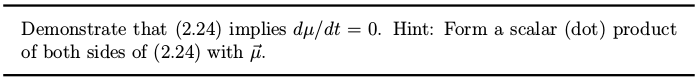
\includegraphics[width=0.8\textwidth,keepaspectratio]{prbl25}
        \label{fig:prbl25}
\end{figure}

\textit{Remember:}
\begin{itemize}
	\item The magnitude of $\vec{\mu}$ does not change in time.
\end{itemize}


\textit{Proof.} \\
Dot product on the right hand side: \\
\begin{flalign*}
    \frac{d\vec{\mu}}{dt} & = \gamma \vec{\mu} \times \vec{B} \\
    \frac{d\vec{\mu}}{dt} \cdot \vec{\mu} & = \gamma (\vec{\mu} \times \vec{B}) \cdot \vec{\mu} \\
    \frac{d\vec{\mu}}{dt} \cdot \vec{\mu} & = (\gamma\, \mu \, B \, 
    sin\theta \, \hat{n}) \cdot \vec{\mu} \\
    \text{Obs: } \hat{n} \text{ is orthogonal to } \vec{\mu} & \Rightarrow cos(\angle( \hat{n}, \vec{\mu})) = 0 \Rightarrow \\
    \frac{d\vec{\mu}}{dt} \cdot \vec{\mu} & = 0 \, (1) \\
\end{flalign*}
Dot product on the left hand side: \\
\begin{flalign*}
    \vec{\mu} \cdot \frac{d\vec{\mu}}{dt} & = \gamma (\vec{\mu} \times \vec{B}) \cdot \vec{\mu} \\
    \vec{\mu} \cdot \frac{d\vec{\mu}}{dt} & = \vec{\mu} \cdot (\gamma\, 
    \mu \, B \, sin\theta \, \hat{n})\\
    \text{Obs: } \hat{n} \text{ is orthogonal to } \vec{\mu} & \Rightarrow cos(\angle( \hat{n}, \vec{\mu})) = 0 \Rightarrow \\
    \vec{\mu} \cdot \frac{d\vec{\mu}}{dt} &= 0 \, (2)\\
\end{flalign*}

From (1) + (2) we get: \\
\begin{flalign*}
	\frac{d\vec{\mu}}{dt} \cdot \vec{\mu} + \vec{\mu} \cdot 
	\frac{d\vec{\mu}}{dt} &= 0 \\
	\frac{d(\vec{\mu} \cdot \vec{\mu})}{dt} &= 0 \\
	\frac{d\mu^2}{dt} &= 0 \\
	\frac{d \mu}{dt} \, \mu + \mu \, \frac{d \mu}{dt} &= 0 \\
	2 \, \mu \, \frac{d \mu}{dt} &= 0 \\
	\frac{d \mu}{dt} &= 0
\end{flalign*}

\clearpage
%%%%%%%%%%%%%%%%%%%%%%%%%%%%%%%
\Large{Problem 2.6}

\begin{figure}[H]
        \centering
        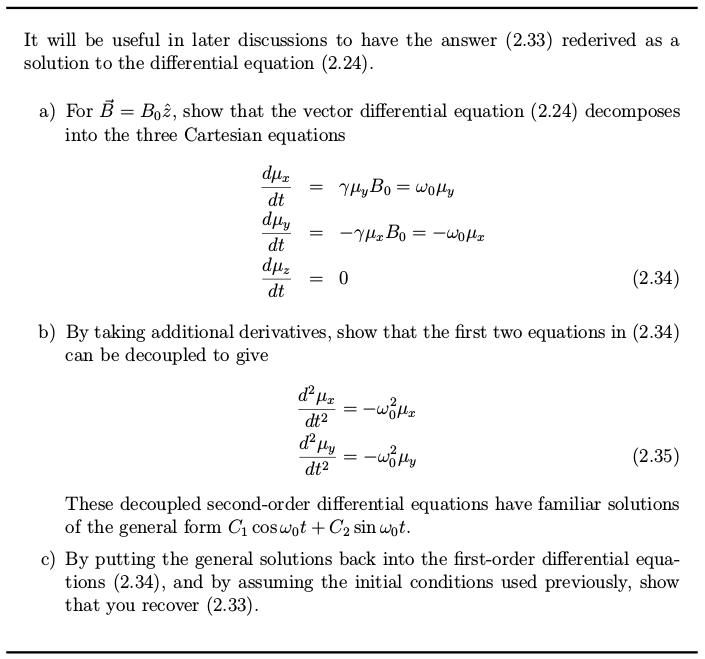
\includegraphics[width=0.8\textwidth,keepaspectratio]{prbl26}
        \label{fig:prbl26}
\end{figure}

\textit{Remember:}
\begin{itemize}
	\item The magnitude of the z-component of the magnetic moment does 
	not change in time, while the xy-components rotate about the z 
	axis.
\end{itemize}

(2.33)
\begin{align*}\label{eq:eq233}
    \vec{\mu_x}(t) & = \vec{\mu_x}(0) \cdot cos \omega_0 t + \vec{\mu_y}(0)   \cdot sin \omega_0 t \\
    \vec{\mu_y}(t) & = \vec{\mu_y}(0) \cdot cos \omega_0 t - \vec{\mu_x}(0)   \cdot sin \omega_0 t \\
    \vec{\mu_z}(t) & = \vec{\mu_z}(0)
\end{align*}

(2.24)
\begin{equation*} 
    \frac{d\vec{\mu}}{dt} = \gamma \vec{\mu} \times      \vec{B}
\end{equation*}

\textit{a) Proof.}
\begin{flalign*}
   \frac{d}{dt} (\vec{\mu_x} + \vec{\mu_y} + \vec{\mu_z} ) & = \gamma (\vec{\mu_x} + \vec{\mu_y} + \vec{\mu_z}) \times (\vec{B_x} + \vec{B_y} + \vec{B_z}) \\
    & = \gamma\, B_0\, (\mu_x \hat{x} + \mu_y \hat{y} + \mu_z\hat{z}) \times \hat{z}\\
    & = \gamma\, B_0\, ( -\mu_x \hat{y} + \mu_y \hat{x}  ) \\
    \frac{d\mu_x}{dt} & = \gamma \mu_y B_0 = \omega_0\,\mu_y \\
    \frac{d\mu_y}{dt} & = - \gamma \mu_x B_0 = - \omega_0\,\mu_x \\
    \frac{d\mu_z}{dt} & = 0
\end{flalign*}

\textit{b) Proof.}
\begin{flalign*}
	\frac{d^2 \mu_x}{dt^2} & = \frac{d}{dt} (\frac{d \mu_x}{dt}) = 
	\omega_0 \frac{d \mu_y}{dt} = -\omega_0^2 \mu_x \\
	\frac{d^2 \mu_y}{dt^2} & = \frac{d}{dt} (\frac{d \mu_y}{dt}) = 
	- \omega_0 \frac{d \mu_x}{dt} = -\omega_0^2 \mu_y \\
\end{flalign*}
%\begin{flalign*}
%   f(t)   &= C_1 \, cos\omega_0 t \, + \, C_2 \, sin \omega_0 t \\
%   f'(t)  &= - C_1 \omega_0 \, sin\omega_0 t + C_2 \omega_0 \, cos \omega_0 t \\
%   f''(t) &= - C_1 \omega_0^2 \, cos\omega_0 t - C_2 \omega_0^2 \, sin \omega_0 t \\
%          & \Rightarrow \\
%   f''(t) &= - \omega_0^2 \, (C_1 \, cos\omega_0 t \, + \, C_2 \, sin \omega_0 t) \\
%   f''(t) &= - \omega_0^2 \, f(t)  \\
%          & \Rightarrow \\
%   \frac{d^2 \mu_x}{dt^2} & = -\omega_0^2 \mu_x \\
%   \frac{d^2 \mu_y}{dt^2} & = -\omega_0^2 \mu_y 
%\end{flalign*}

\textit{c) Proof.}
\begin{flalign*}
   f(t)   &= C_1 \, cos\omega_0 t \, + \, C_2 \, sin \omega_0 t \\
   f(0)   &= C_1 & \Rightarrow C_1 = f(0) \\
   f'(t)  &= - C_1 \omega_0 \, sin\omega_0 t + C_2 \omega_0 \, cos \omega_0 t \\
   f'(0)  &= C_2 \omega_0 & \Rightarrow C_2 = \frac{f'(0)}{\omega_0} \\ \\
\end{flalign*}
\begin{flalign*}
   \mu_x(t) &= C_{1x} \, cos\omega_0 t + C_{2x} sin \omega_0 t \\
   C_{1x} &= \mu_x(0) \\
   C_{2x} &= \frac{d\mu_x(0)}{dt} \frac{1}{\omega_0} = \mu_y(0) \\
          & \Rightarrow \\
   \mu_x(t) &= \mu_x(0) \, cos\omega_0 t + \mu_y(0) sin \omega_0 t \\ \\
\end{flalign*}
\begin{flalign*}
   \mu_y(t) &= C_{1y} \, cos\omega_0 t + C_{2y} sin \omega_0 t \\
   C_{1y} &= \mu_y(0) \\
   C_{2y} &= \frac{d\mu_y(0)}{dt} \frac{1}{\omega_0} = - \mu_x(0) \\
          & \Rightarrow \\
   \mu_y(t) &= \mu_y(0) \, cos\omega_0 t - \mu_x(0) sin \omega_0 t \\ \\
   \mu_z(t) &= \mu_z(0)
\end{flalign*}


\clearpage
%%%%%%%%%%%%%%%%%%%%%%%%%%%%%%%
\Large{Problem 2.7}

\begin{figure}[H]
        \centering
        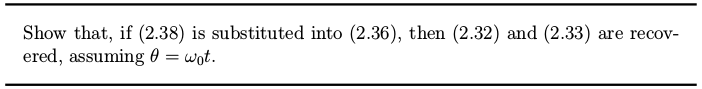
\includegraphics[width=0.8\textwidth,keepaspectratio]{prbl27}
        \label{fig:prbl27}
\end{figure}

\textit{Remember:}
\begin{itemize}
	\item The precession motion of a particle placed in a static 
	magnetic field can be described using a matrix representation.
\end{itemize}

\textit{Proof.}
\begin{flalign*}
\vec{\mu}(t) & = 
\begin{pmatrix}
cos\theta & sin\theta & 0 \\
-sin\theta & cos\theta & 0 \\
0 & 0 & 1
\end{pmatrix}
\cdot \vec{\mu}(0)\\
\begin{pmatrix}
\mu_x(t)\\
\mu_y(t)\\
\mu_z(t)
\end{pmatrix}
& =
\begin{pmatrix}
cos\theta & sin\theta & 0 \\
-sin\theta & cos\theta & 0 \\
0 & 0 & 1
\end{pmatrix}
\cdot
\begin{pmatrix}
\mu_x(0)\\
\mu_y(0)\\
\mu_z(0)
\end{pmatrix}
\Rightarrow \\
    {\mu_x}(t) &= {\mu_x}(0) \cdot cos \omega_0   t + {\mu_y}(0) \cdot sin \omega_0 t \\
    {\mu_y}(t) &= {\mu_y}(0) \cdot cos \omega_0   t - {\mu_x}(0) \cdot sin \omega_0 t \\
    {\mu_z}(t) &= {\mu_z}(0)
\end{flalign*}


\clearpage
%%%%%%%%%%%%%%%%%%%%%%%%%%%%%%%
\Large{Problem 2.8}

\begin{figure}[H]
        \centering
        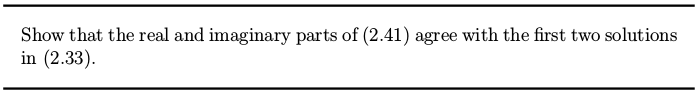
\includegraphics[width=0.8\textwidth,keepaspectratio]{prbl28}
        \label{fig:prbl28}
\end{figure}

\textit{Remember:}
\begin{itemize}
	\item The 2 degrees of freedom, $\mu_x$ and $\mu_y$ can be given 
	in terms of real and imaginary part of $\mu_+$.
	\item Phase directly relates to position and is of utmost 
	importance in the description of spin motion.
\end{itemize}

\textit{Proof.}
\begin{flalign*}
    {\mu_{+}}(t) & = {\mu_{+}}(0) e^{-i\omega_0t}\\
    & = (\mu_{x}(0) + i\, \mu_{y}(0)) \, e^{-i\omega_0t} \\
    & = (\mu_{x}(0) + i\, \mu_{y}(0)) \, (cos\omega_0 t \, - \, i \, sin\omega_0t) \\
    & = \mu_{x}(0) \, cos\omega_0 t - i\, \mu_{x}(0) \, sin\omega_0t + i\, \mu_{y}(0) \, cos\omega_0 t + \mu_{y}(0) sin\omega_0t \\
    & = \mu_x(t) + i \, \mu_y(t)
\end{flalign*}

\clearpage
%%%%%%%%%%%%%%%%%%%%%%%%%%%%%%%
%\Large{Whiteboard Problems}
%
%\begin{figure}[H]
%    \centering
%    \includegraphics[width=0.8\textwidth,keepaspectratio]{Ch2Gary1}
%    \label{fig:Ch2Gary1}
%\end{figure}
%
%\begin{figure}[H]
%    \centering
%    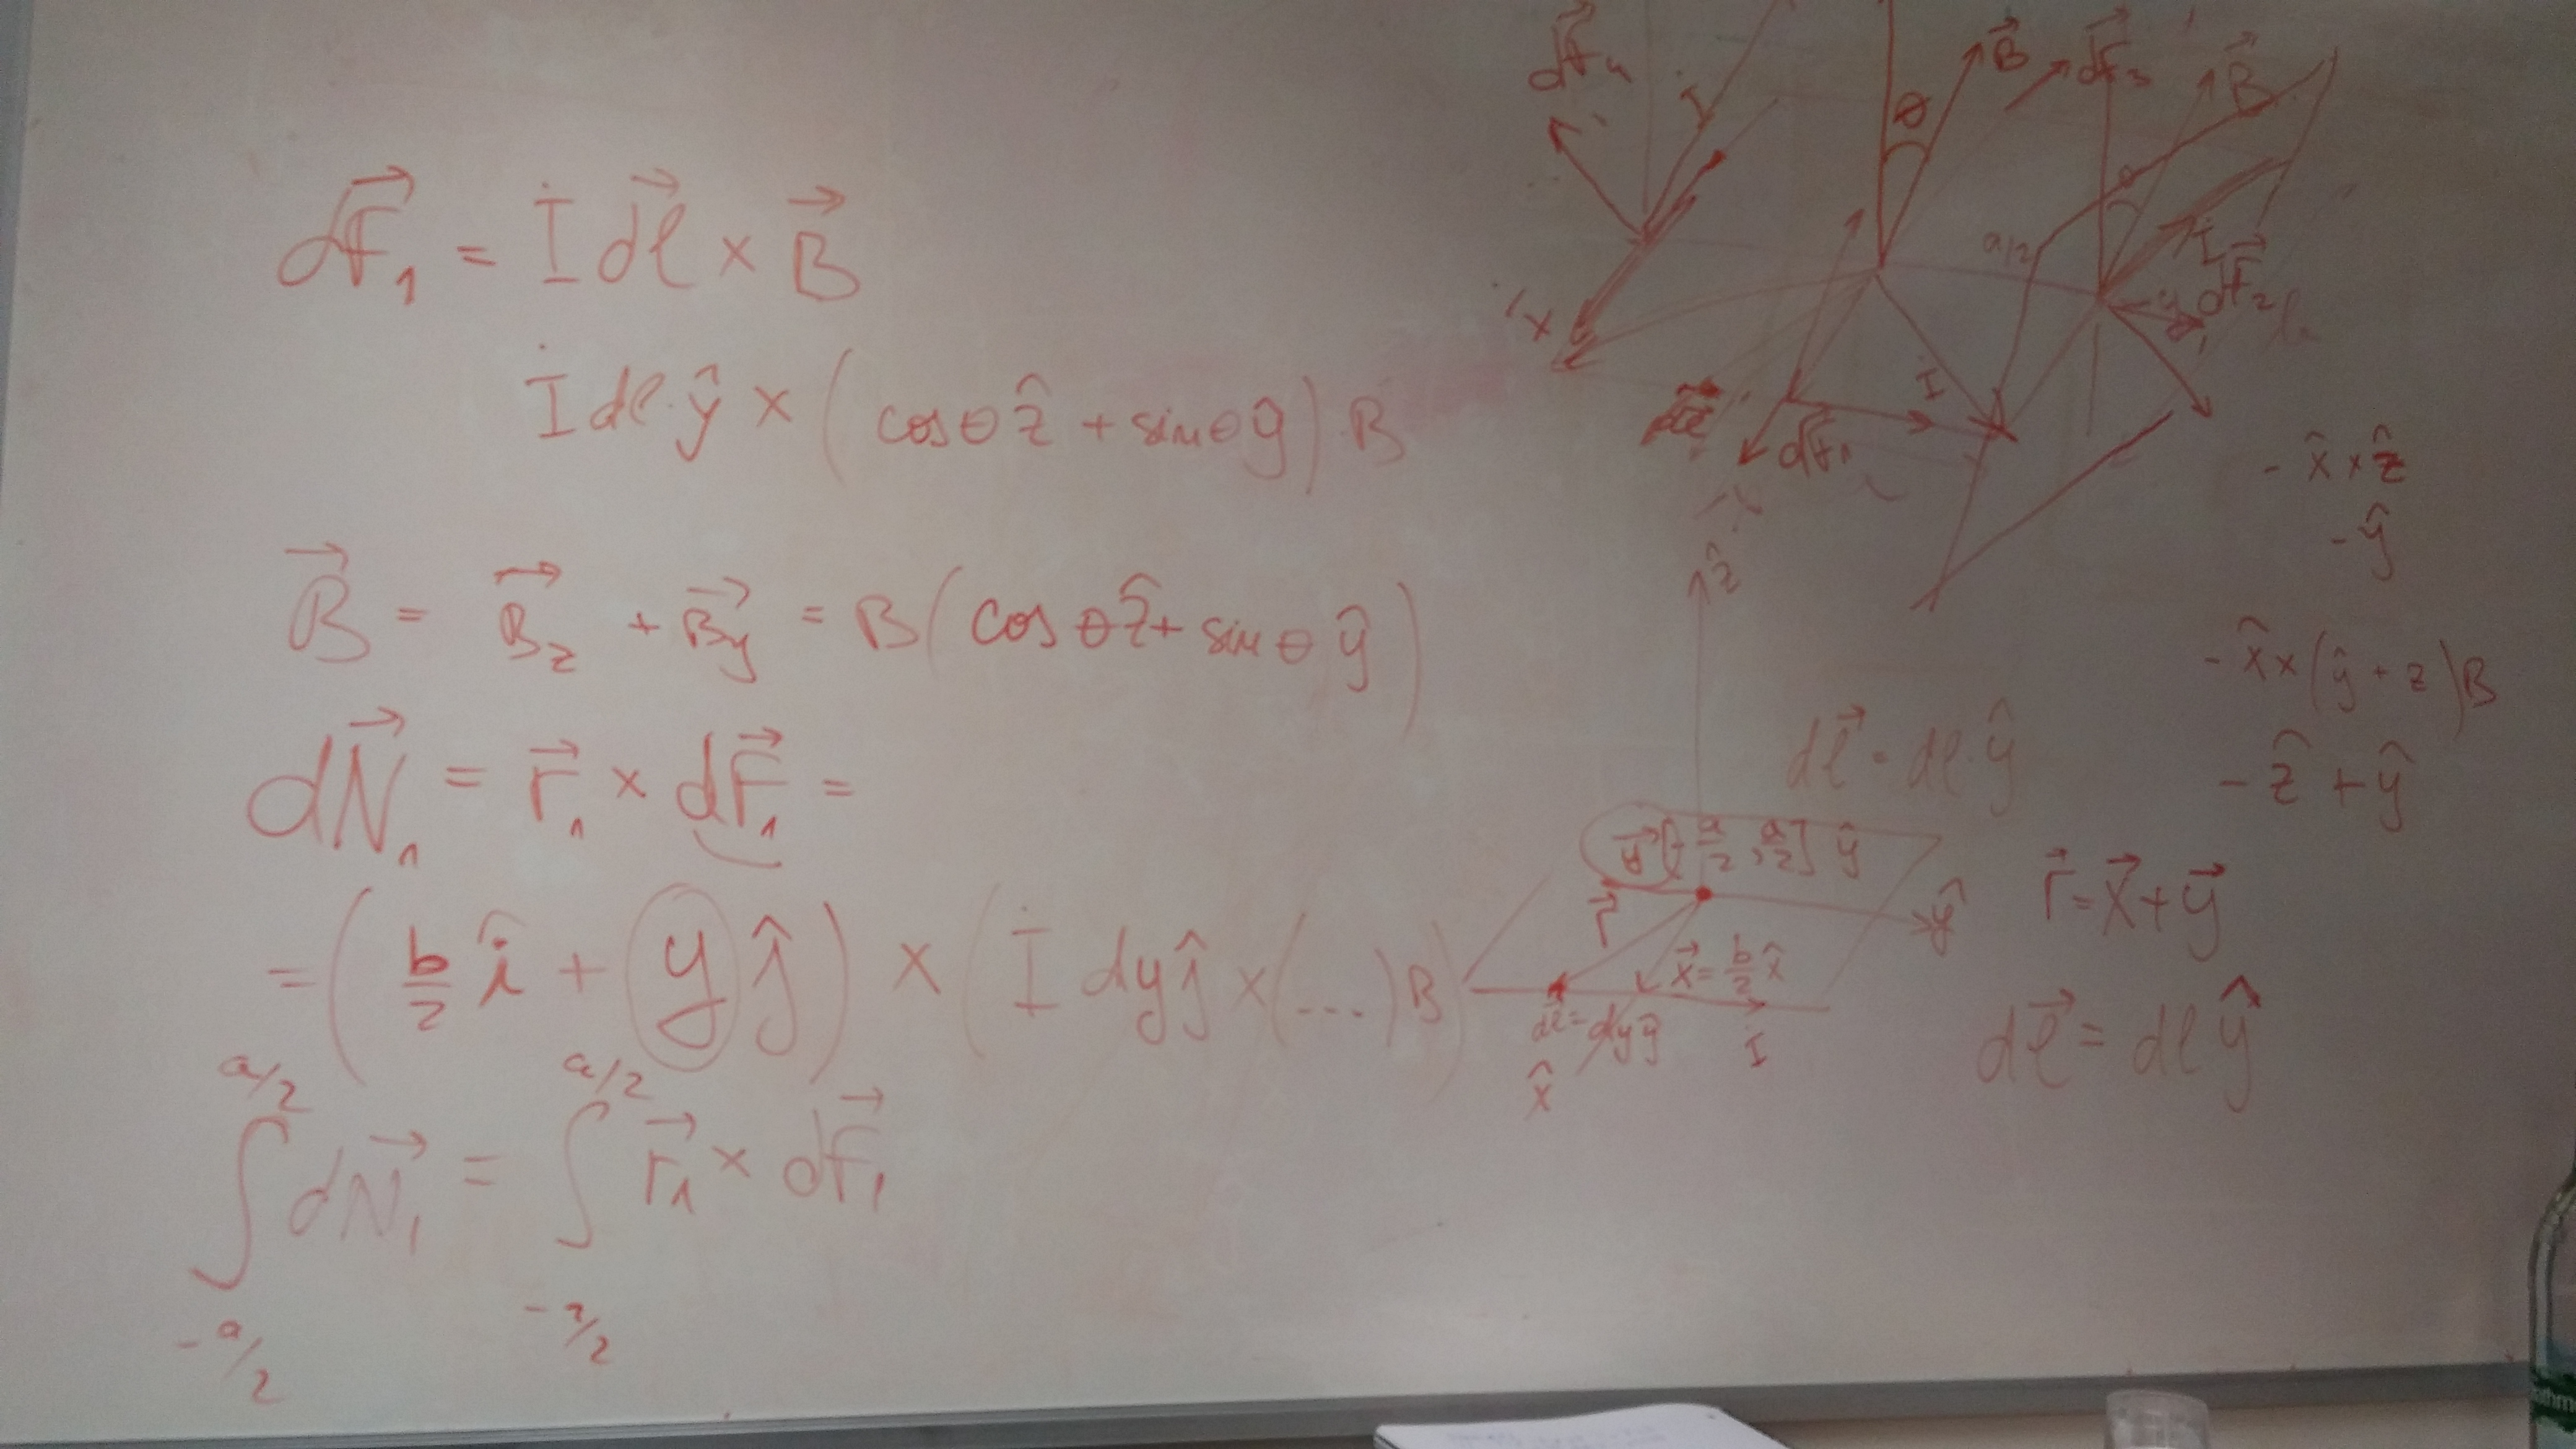
\includegraphics[width=0.8\textwidth,keepaspectratio]{Ch2Gary2}
%    \label{fig:Ch2Gary2}
%\end{figure}
%
%\begin{figure}[H]
%    \centering
%    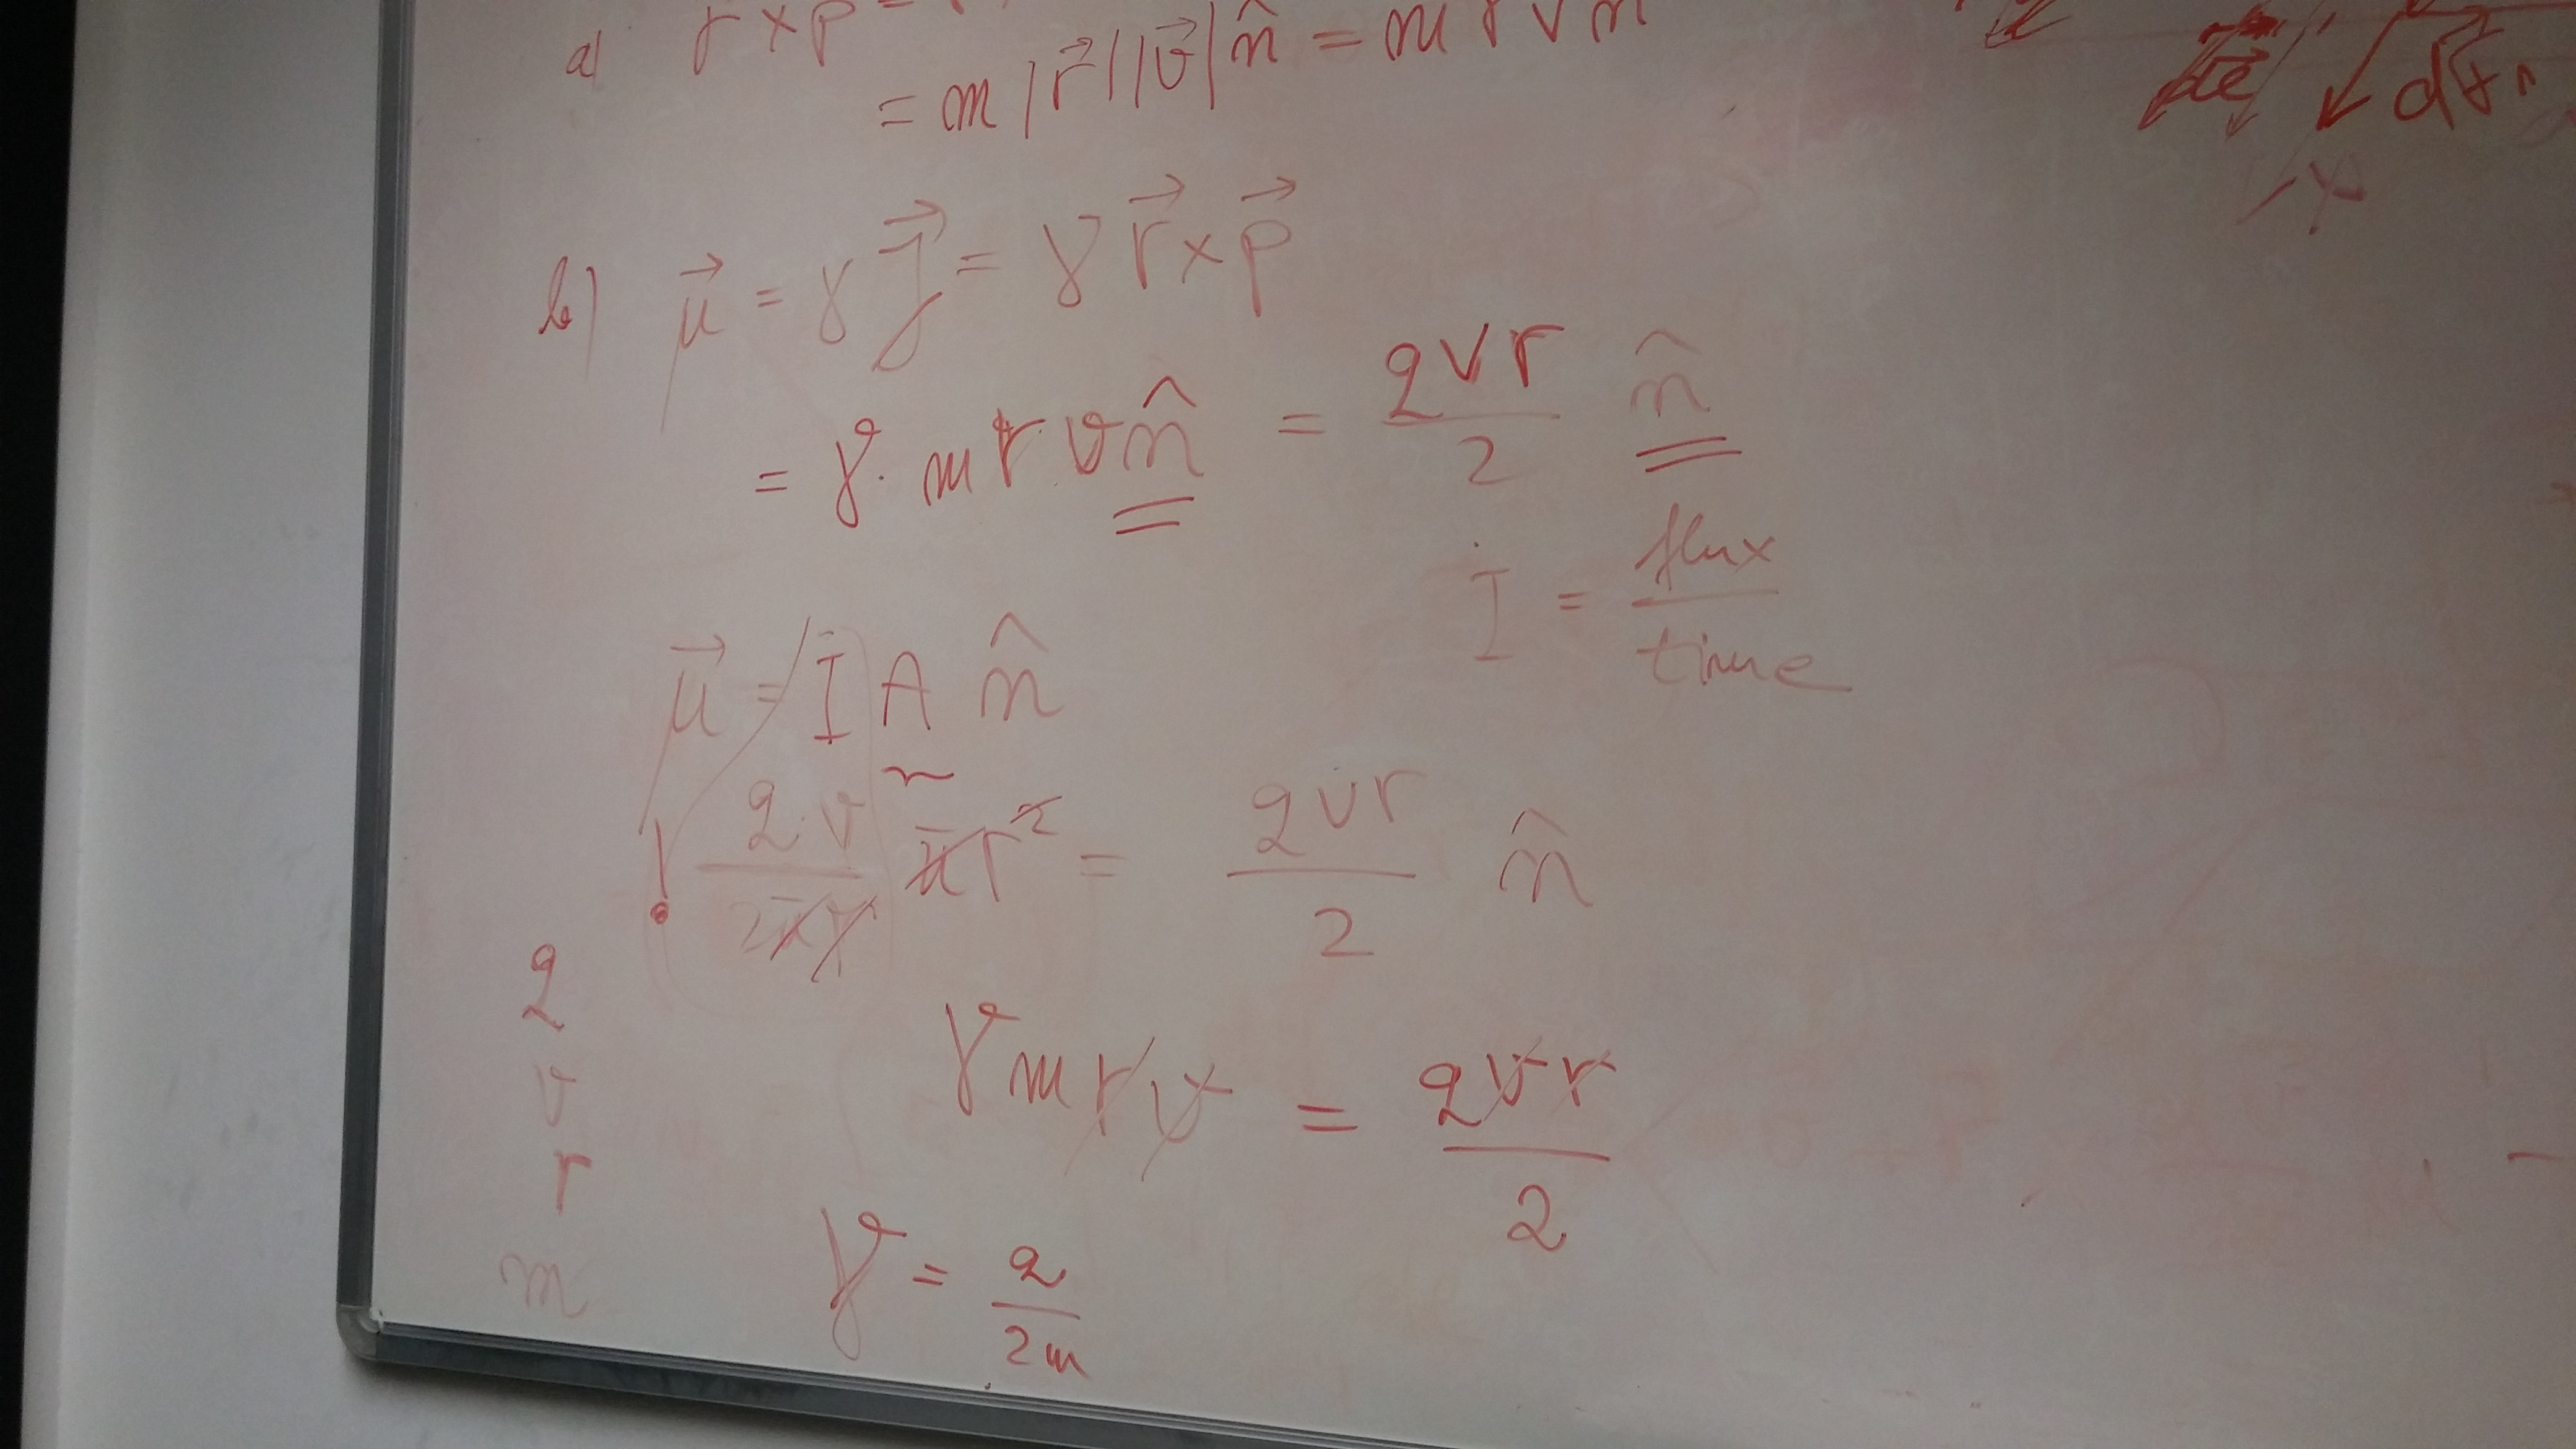
\includegraphics[width=0.8\textwidth,keepaspectratio]{Ch2Gary3}
%    \label{fig:Ch2Gary3}
%\end{figure}
%
%\begin{figure}[H]
%    \centering
%    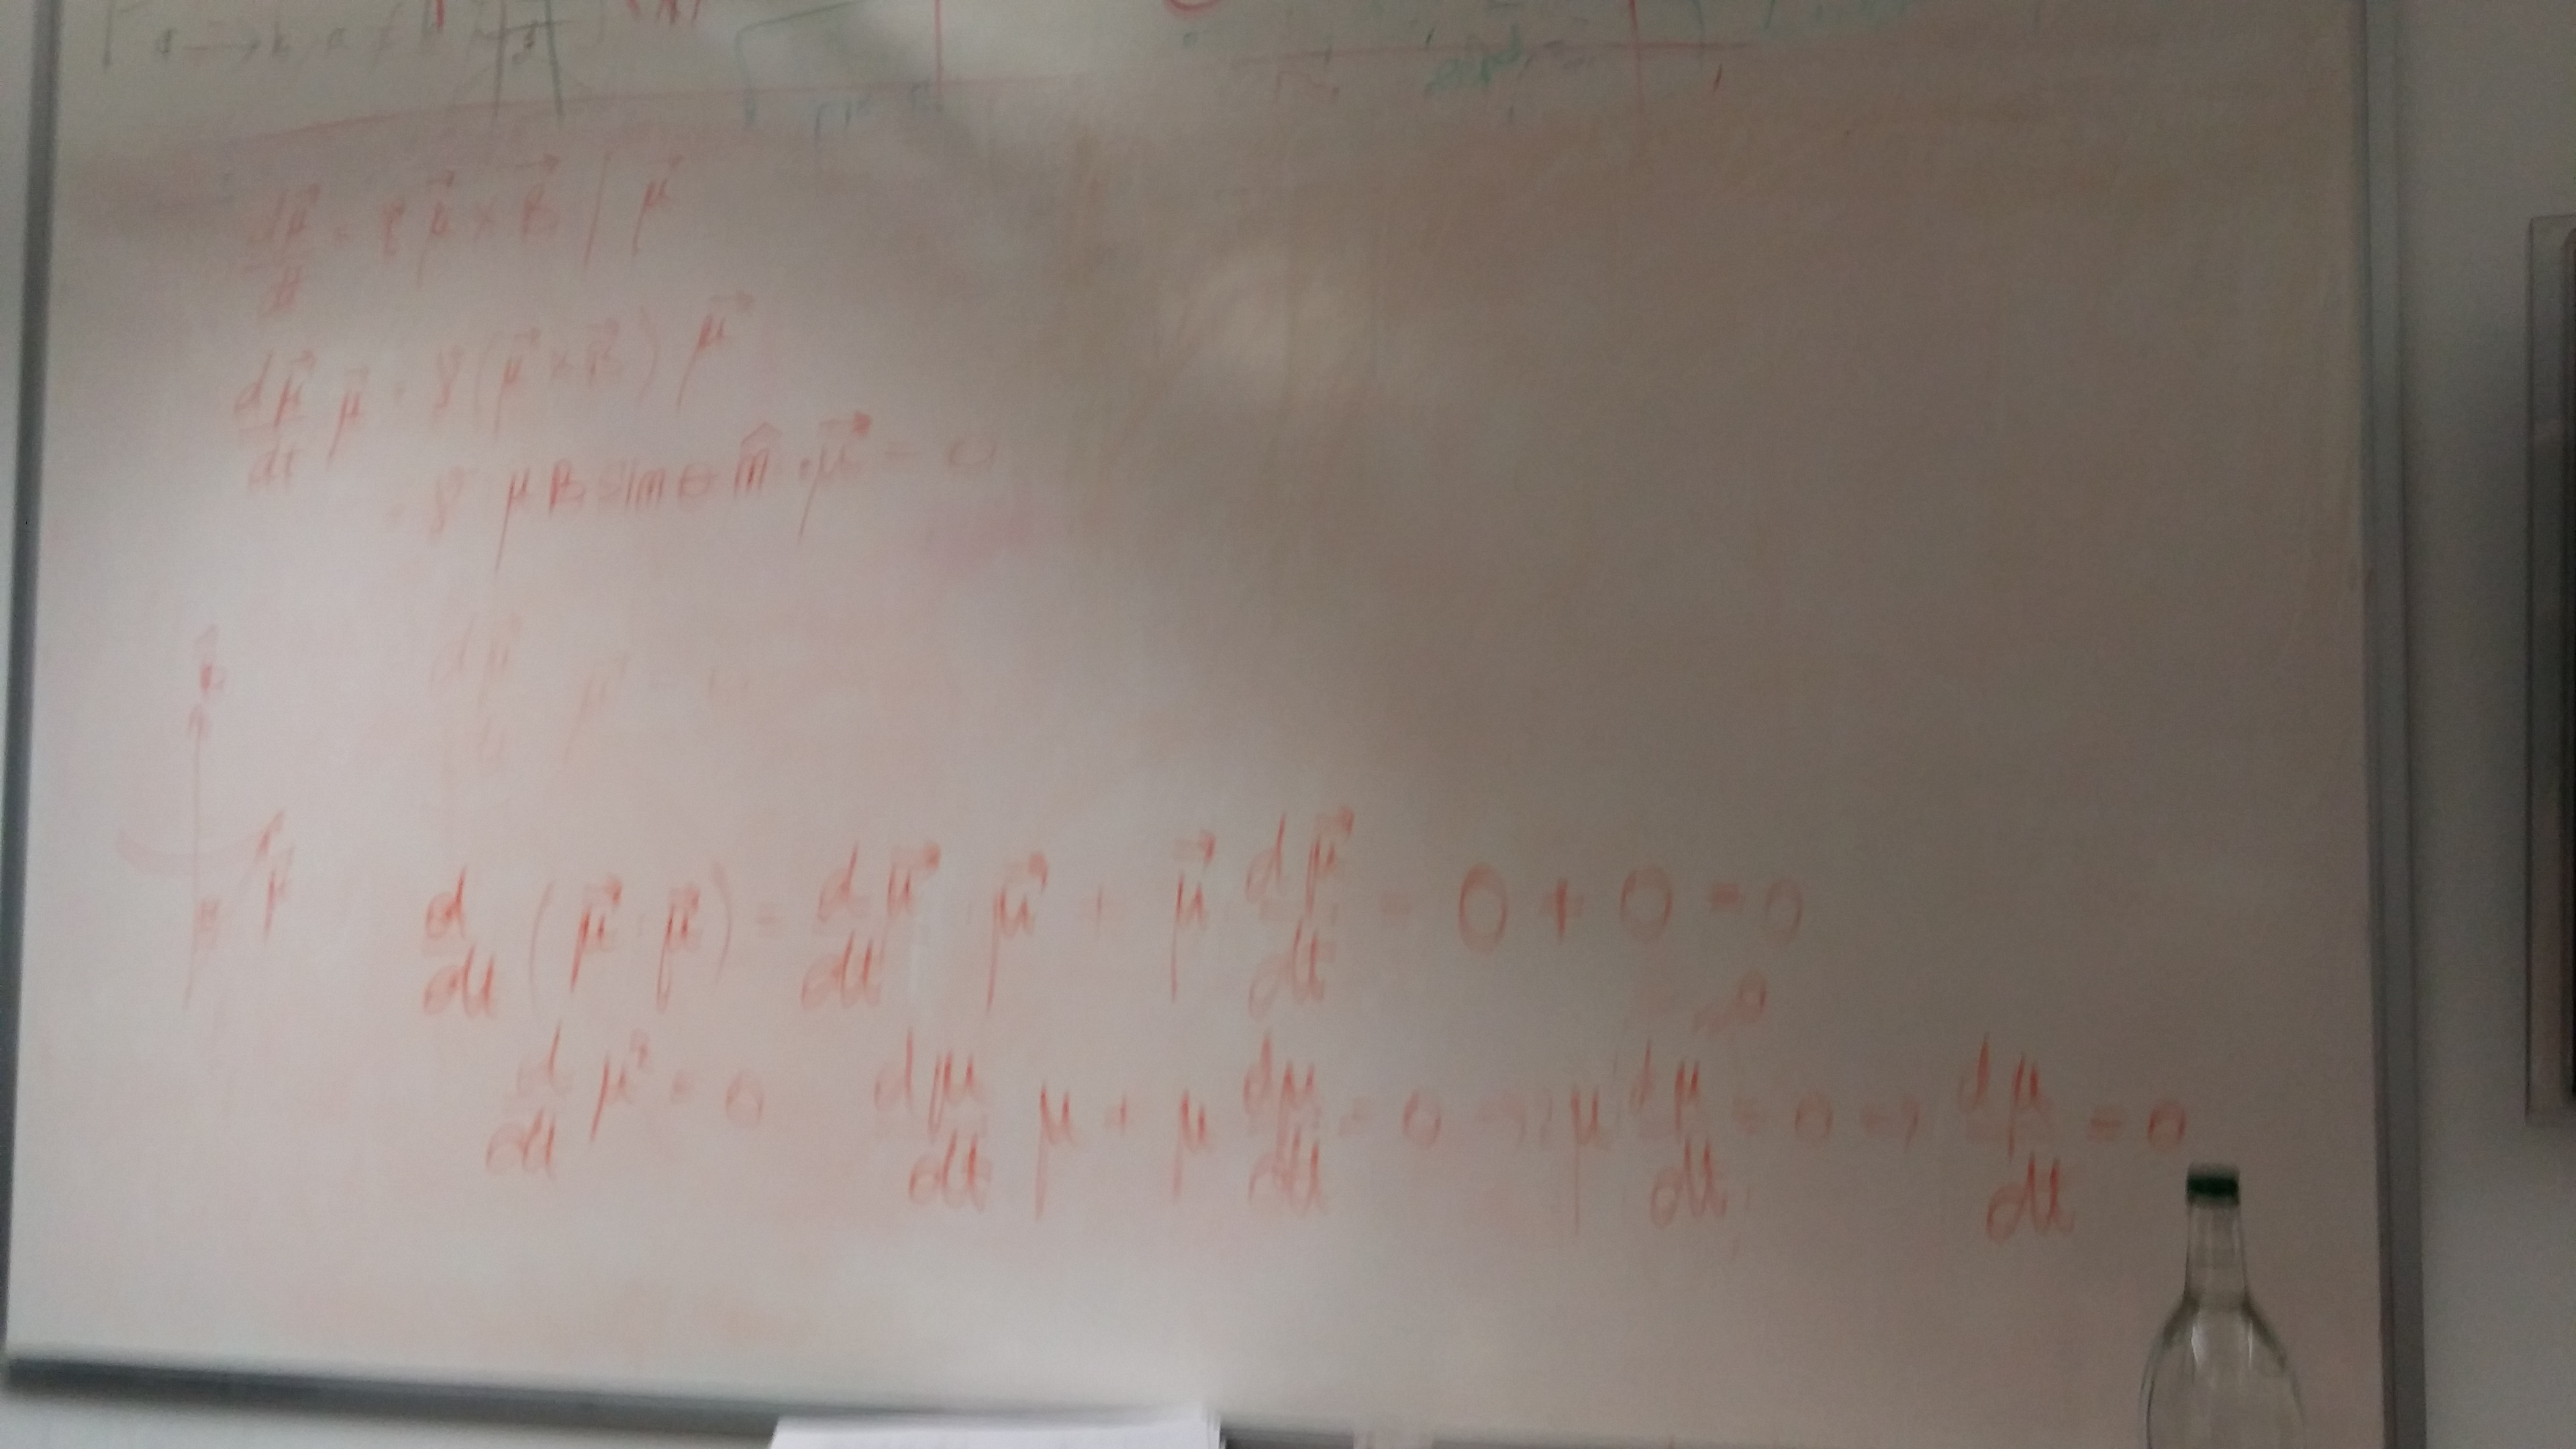
\includegraphics[width=0.8\textwidth,keepaspectratio]{Ch2Gary4}
%    \label{fig:Ch2Gary4}
%\end{figure}
%
%\begin{figure}[H]
%    \centering
%    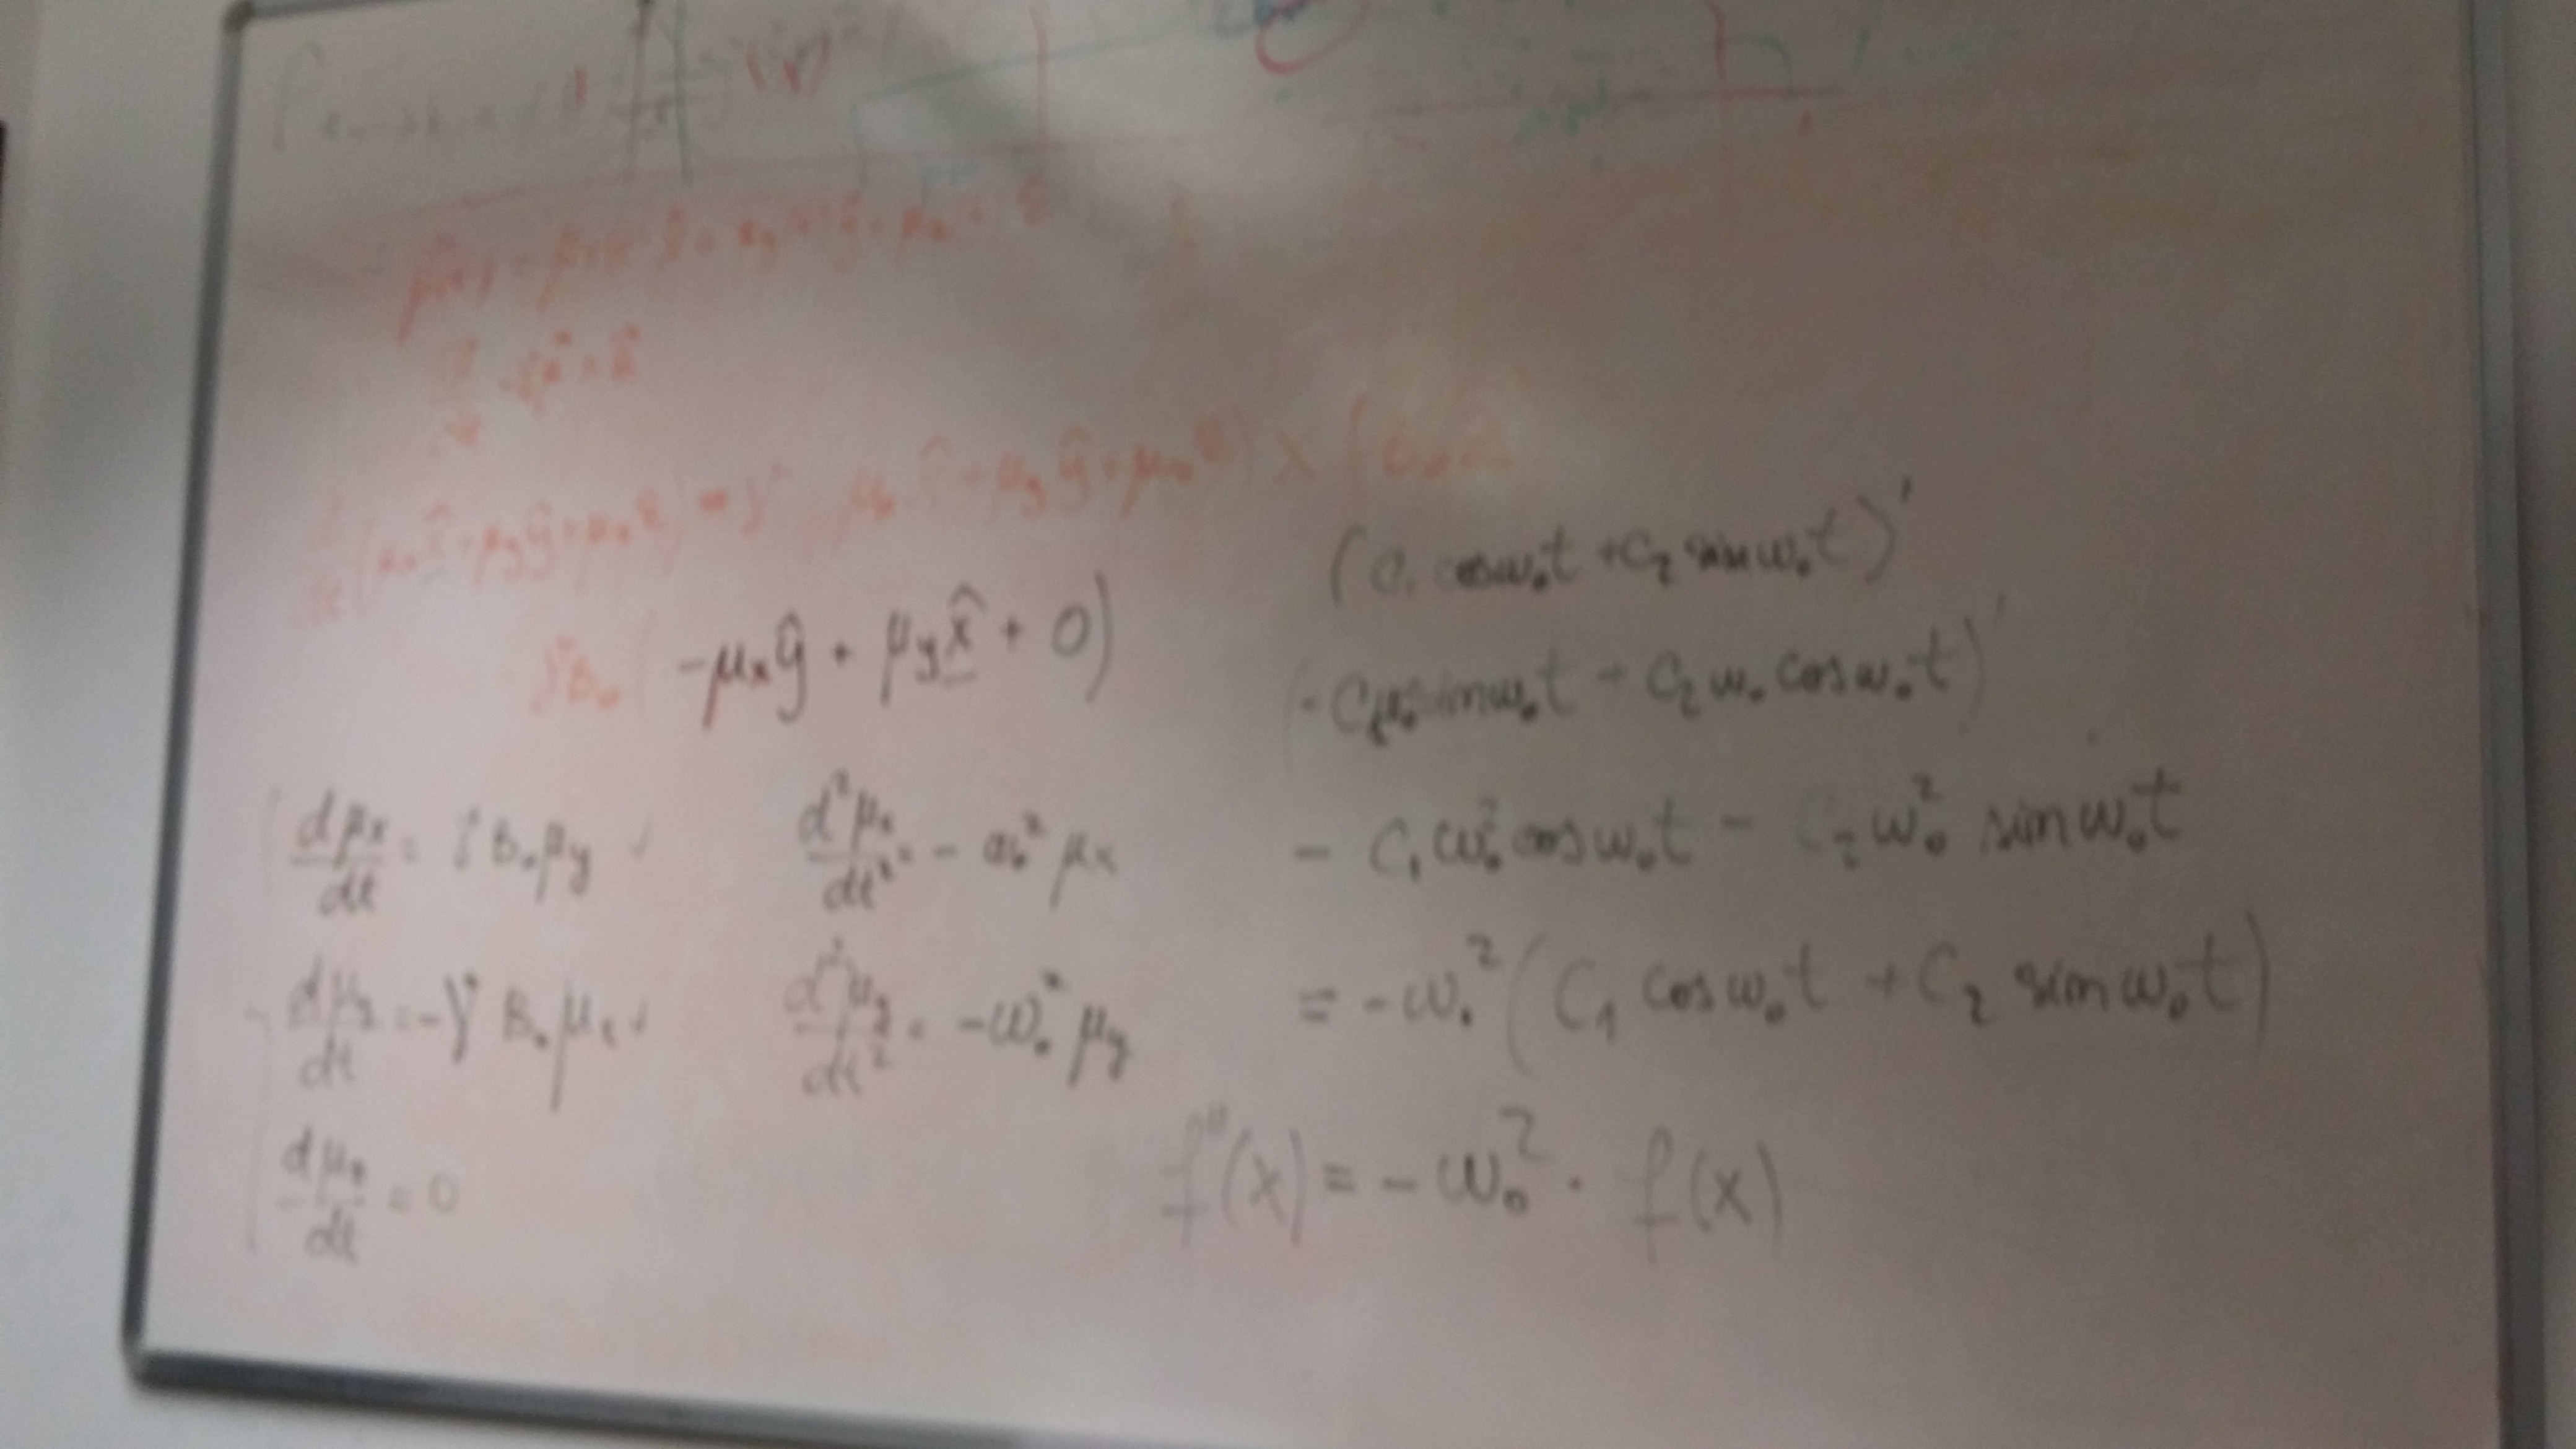
\includegraphics[width=0.8\textwidth,keepaspectratio]{Ch2Gary5}
%    \label{fig:Ch2Gary5}
%\end{figure}
%
%\begin{figure}[H]
%    \centering
%    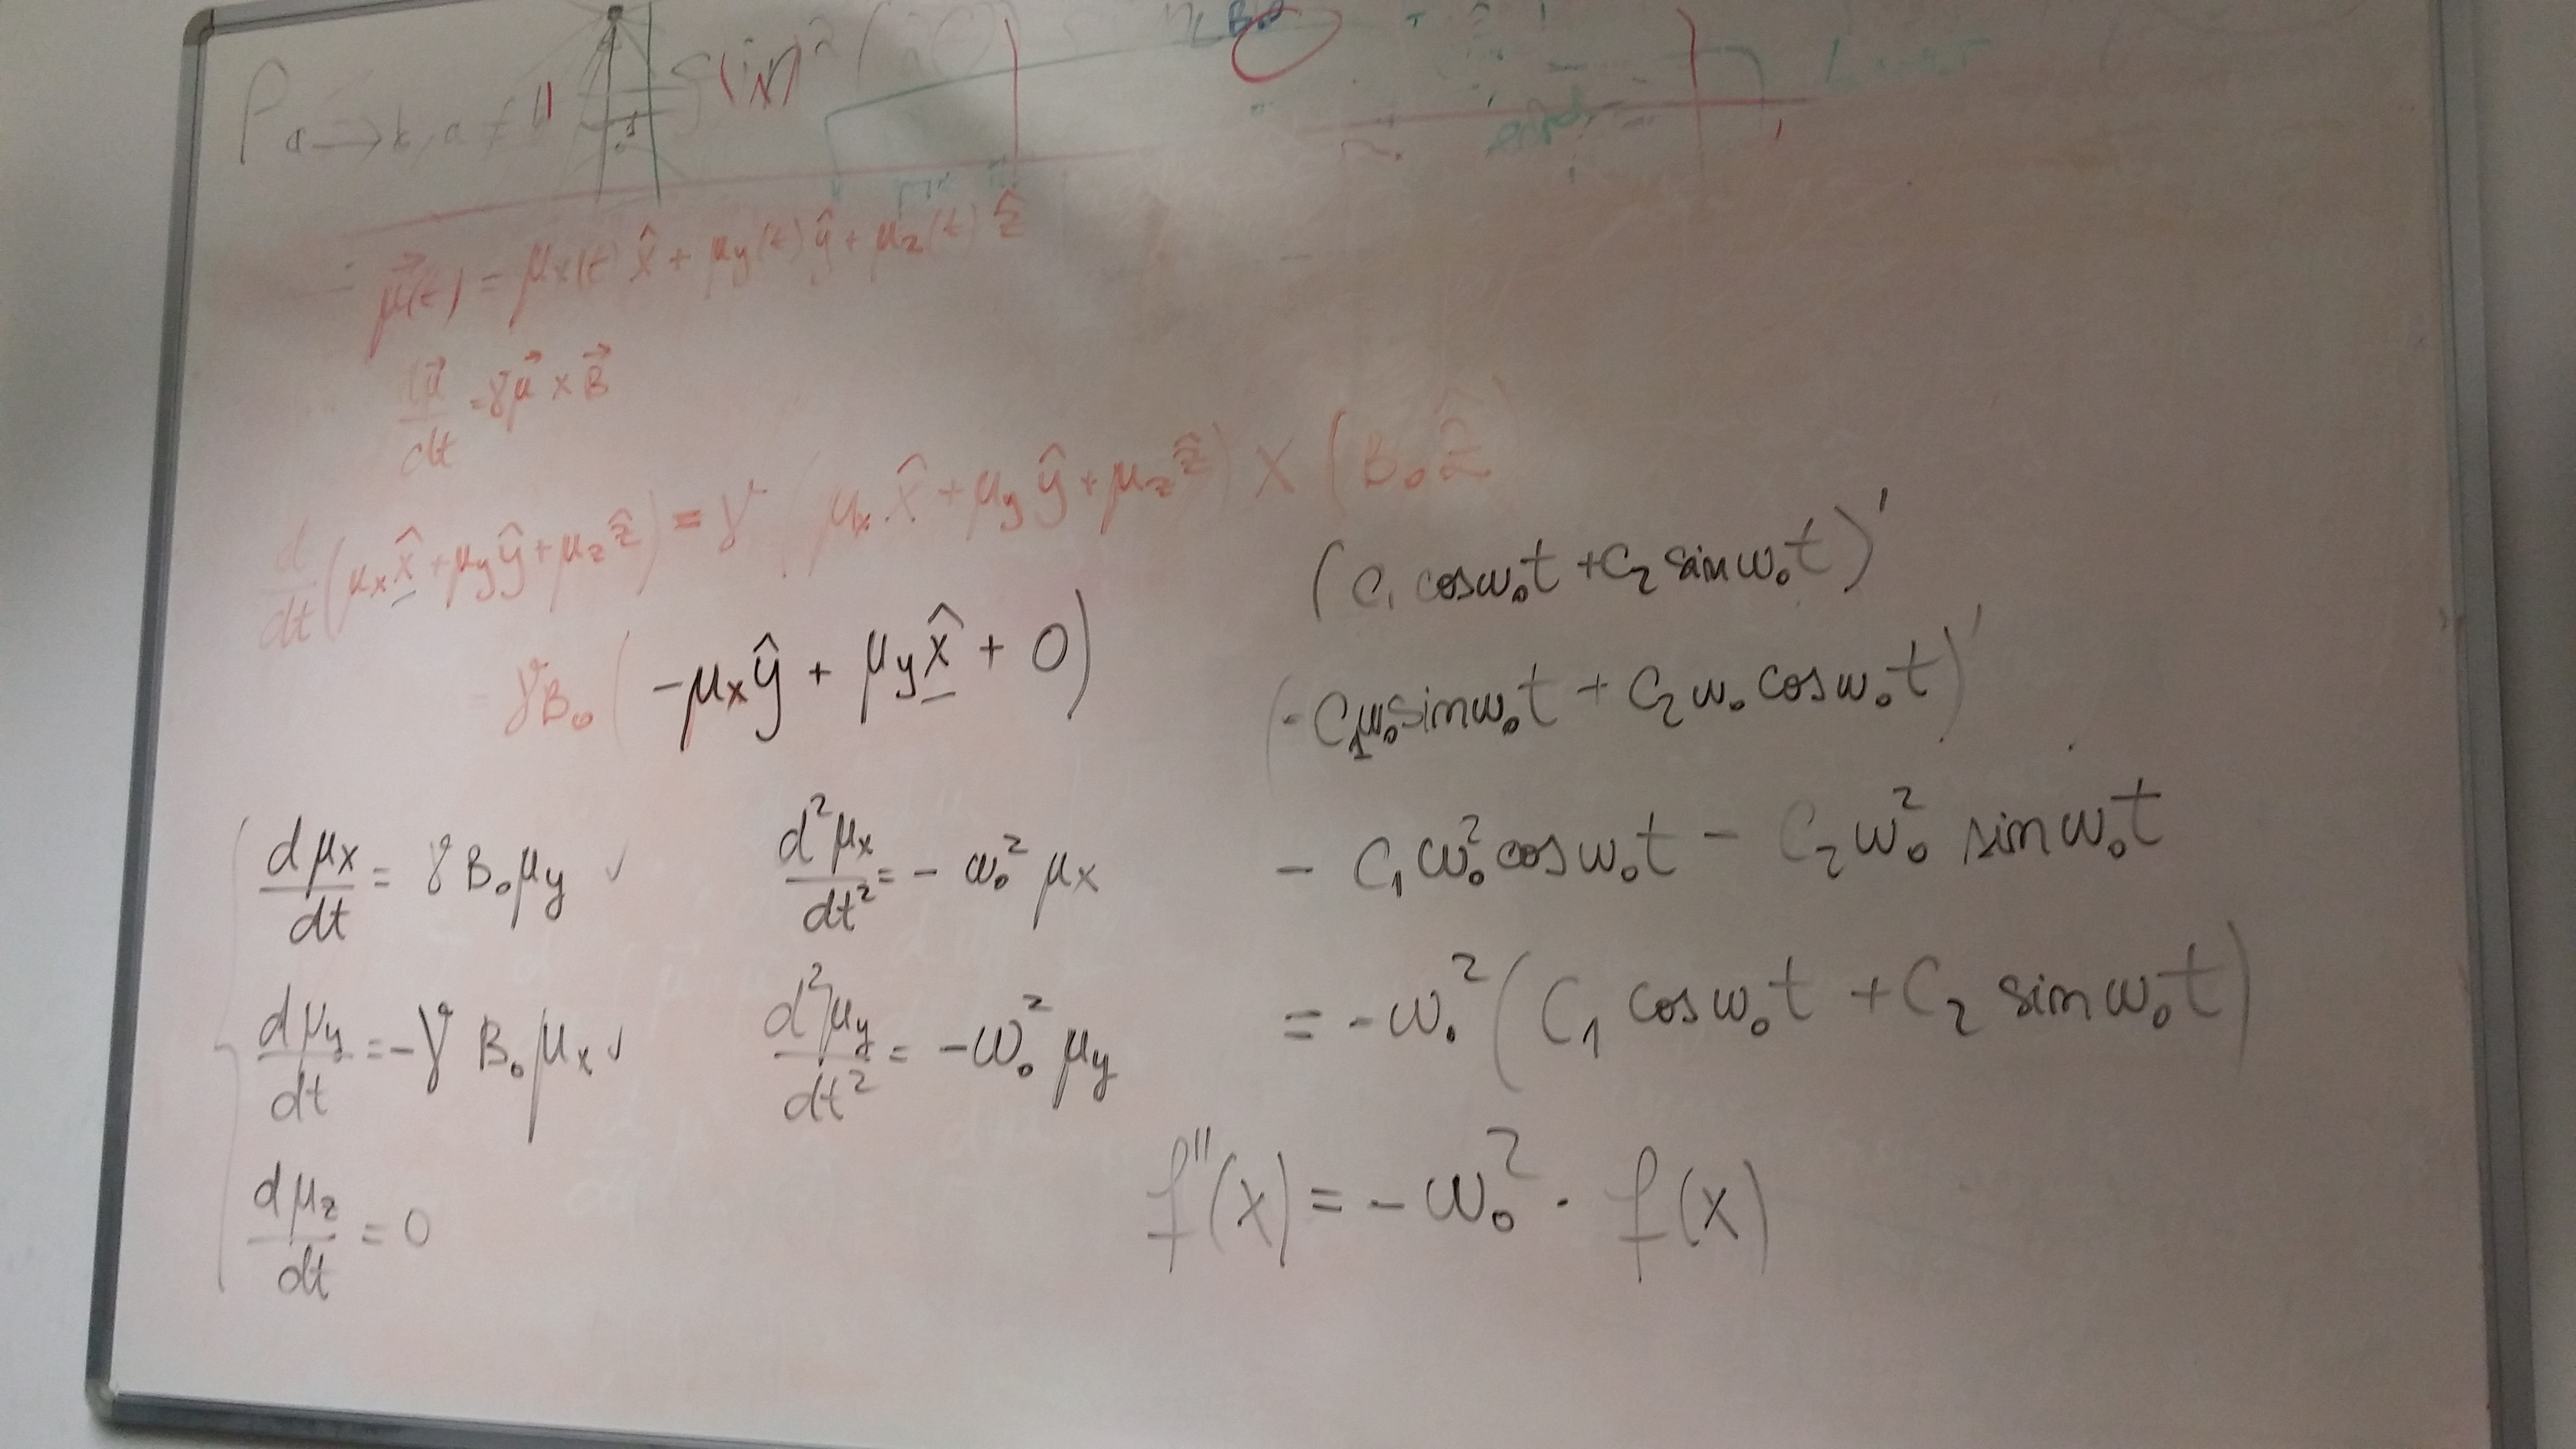
\includegraphics[width=0.8\textwidth,keepaspectratio]{Ch2Gary6}
%    \label{fig:Ch2Gary6}
%\end{figure}
%
%\begin{figure}[H]
%    \centering
%    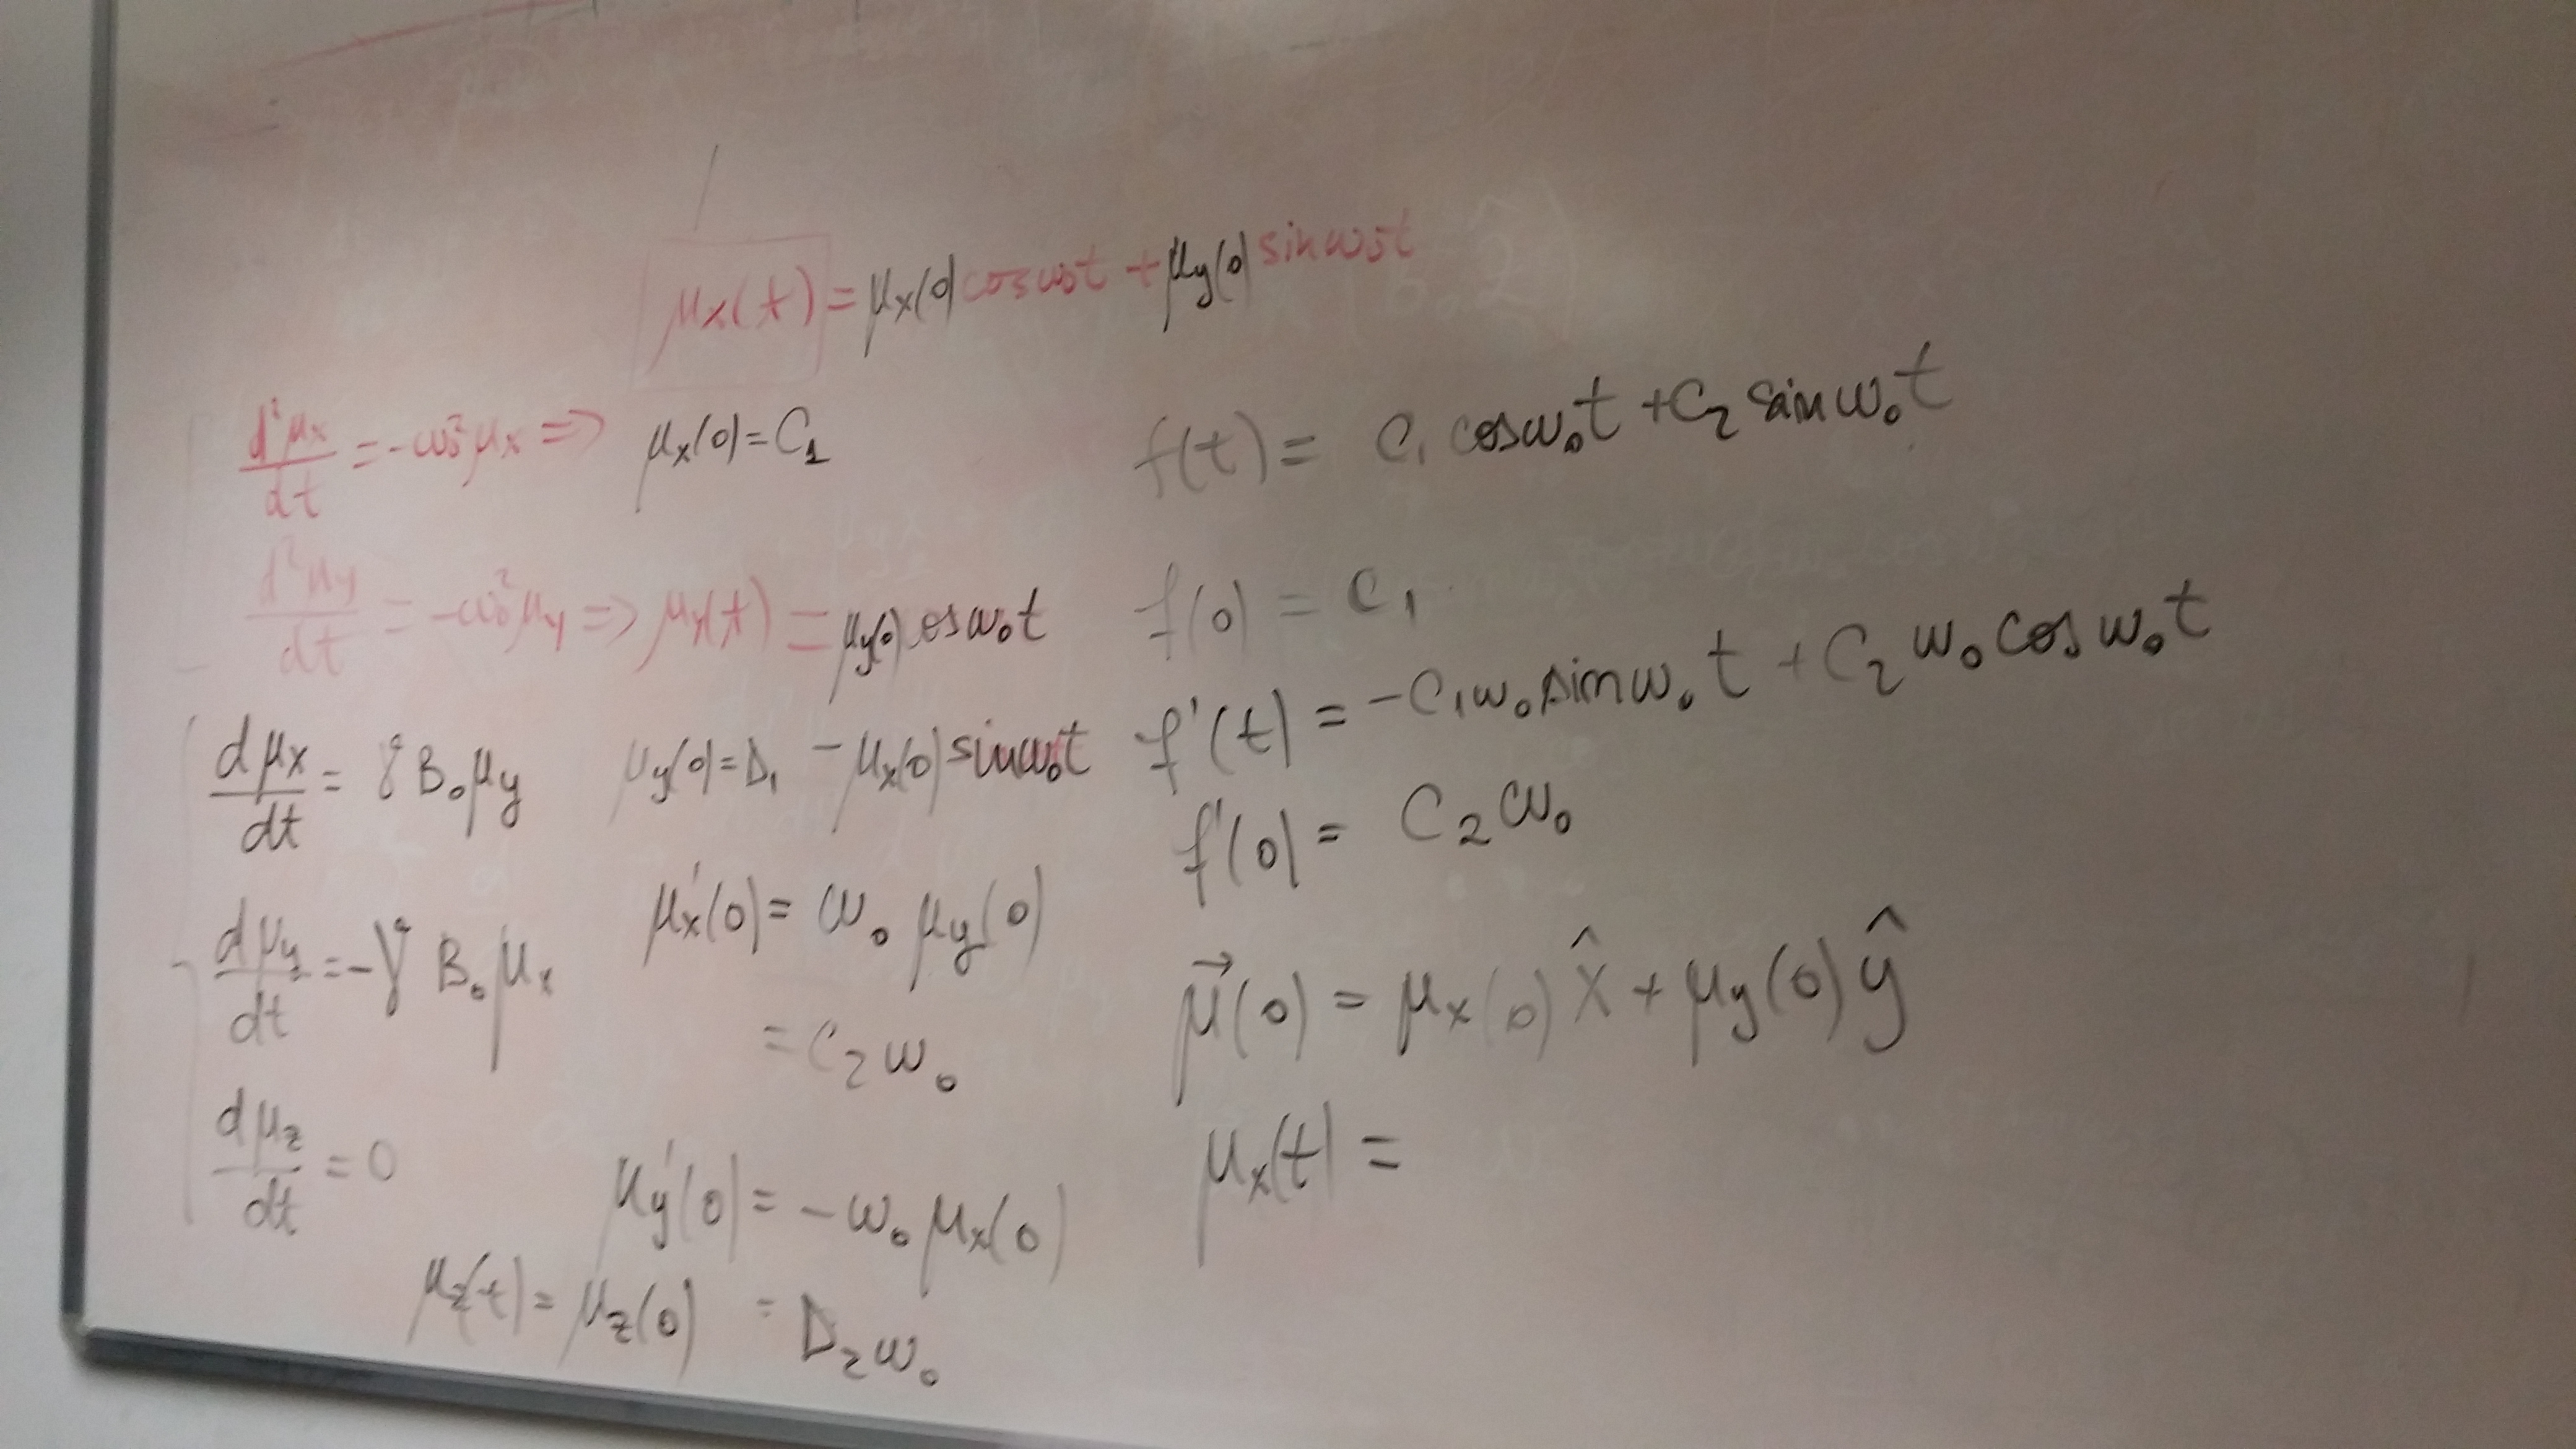
\includegraphics[width=0.8\textwidth,keepaspectratio]{Ch2Gary7}
%    \label{fig:Ch2Gary7}
%\end{figure}
%












